\documentclass[a4paper, 10pt]{article}

\usepackage[margin=1in, bottom=1in]{geometry}
\usepackage{amsmath, amssymb, amsthm}
\usepackage{setspace}
\usepackage{graphicx}
\usepackage{enumitem}
\usepackage{kotex}
\usepackage{subcaption}
\usepackage{hhline}
\usepackage{xcolor}
\usepackage{url}
\usepackage{listings}
\usepackage{courier}
\usepackage[htt]{hyphenat}



\setstretch{1.25}

\newcommand*\justify{%
  \fontdimen2\font=0.4em% interword space
  \fontdimen3\font=0.2em% interword stretch
  \fontdimen4\font=0.1em% interword shrink
  \fontdimen7\font=0.1em% extra space
  \hyphenchar\font=`\-% allowing hyphenation
}

%\renewcommand\refname{참고문헌}
% Referencing Style
\let\OLDthebibliography\thebibliography
\renewcommand\thebibliography[1]{
  \OLDthebibliography{#1}
  \setlength{\parskip}{0em}
  \setlength{\itemsep}{0.4em}
  \setstretch{1}
}

\setlist[itemize]{noitemsep}
\setlist[enumerate]{noitemsep}

\renewcommand{\vec}{\mathbf}


\title{Noisy Student Self-Training on CIFAR-10}
\author{컴퓨터공학부 2016-15523 송우성}
%\date{}

\begin{document}

\maketitle

\section{Noisy Student Self-Training}
준 지도학습(semi-supervised learning)이란 학습에서 목표값이 표시된(labeled)
데이터와 그렇지 않은(unlabeled) 데이터를 함께 사용하는 과정을 의미한다. 모든
데이터의 라벨이 표시된 지도학습(supervised learning)과 달리 학습 과정에서 여러
불확실성을 마주하게 된다. 하지만 수백만개의 모든 데이터에 일일이 태그를 다는데
걸리는 노동과 자원을 절약할 수 있으므로 더 경제적이고 범용적인 방법으로 볼 수
있다. \cite{zhu2006semisupervised}

Self-training은 준 지도학습을 수행하는 한 가지 방법이다. 우선 labeled 데이터만
가지고 모델을 학습하여 unlabeled 데이터에 대한 예측을 한다. 이를 기반으로 pseudo
label을 만들어서 학습을 하고, 다시 예측으로 라벨을 생성하는 과정을 반복한다.
적은 수의 labeled 데이터만으로 학습한 모델은 오류율이 높으므로 생성된 pseudo
label을 온전히 신뢰할 수 없다. 그러므로 일정 confidence threshold를 두고, 이를
넘는 것에 대해서만 학습 데이터에 추가하여 학습을 진행한다. 이는 가장 초기의 준
지도학습 구현 모델이며, 현재까지도 널리 쓰이는 방법 중 하나이다.
\cite{zhu2006semisupervised}

ImageNet 분류기의 구현으로써, 당시 SOTA의 top-1 정확도 기록을 상회하여(88.4\%)
화제가 되었던 teacher-noisy student 모델에 대한 논문이 있었다.
\cite{xie2020selftraining} Teacher와 student 두 모델을 두어, teacher가 생성한
pseudo label을 통해 student model이 학습을 하는 self-training 방식이었다. 특이한
점은 student model을 teacher보다 같거나 더 커다란 네트워크로 구축하여, 학습에
대한 잠재성을 높였다는데 있다. 또한 teacher 모델과 달리 student에만 강력한
노이즈를 두어, student는 teacher보다 더 어려운 방식으로 학습하도록 강제하였다.
저자는 이 방식이 teacher에서 student로 거듭 전수할수록 지식이 팽창되는 knowledge
expansion 철학을 두었음을 강조하였으며, 이는 네트워크 경량화를 위해 사용된
knowledge distillation과는 \cite{hinton2015distilling} 반대 방향임을 언급했다.

Student model에 두 가지 종류의 noise를 제안하였다. 첫째, 데이터 증식에 사용한
input noise가 있다. 이는 이미지 분류에서 높은 효과를 보였던 RandAugment 방법이
\cite{cubuk2019randaugment} 대표적이다. 이것이 적용되지 않은 상태의 이미지를
분류하는 teacher은 깨끗한 pseudo label을 생성하고, student는 더 어려운 학습
과정을 거치게 된다. 둘째, model 자체에 들어간 noise이다. 이는 ResNet과 같은 skip
connection을 지원하는 네트워크에 사용할 수 있는 stochastic depth와
\cite{huang2016deep}, 마지막 분류기에 넣기 위해 거치는 fully connected network에
추가하는 dropout이 있다. 이를 통해 학습 과정에서는 single model처럼 작동하지만,
pseudo label을 생성하거나 최종 분류를 하는 추론 과정에서는 마치 ensemble처럼
작동이 가능했다고 저자는 설명했다. \cite{xie2020selftraining}

최근 이미지 분류기에 커다란 강직성을 주는 데이터 제공 방식으로 label smoothing
\cite{szegedy2015rethinking} 이나 mixup \cite{zhang2018mixup} 등이 많이 적용되고
있다. 전자는 잘못된 label에 대한 가능성을 두고, 답으로 여겨지는 클래스가 아닌
것들에도 일부 점수를 주는 방식이다. 후자는 학습 데이터를 여러 이미지와 label을
혼합하여 구성하는 방법이다. 이를 통해 학습 데이터에 대한 더 generalized model을
습득할 수 있으며, FGSM과 같은 adversarial attack에 대해서 강직하게 된다고 한다.
\cite{zhang2018mixup}

이번 프로젝트에서 나는 noisy student self-training의 소개 논문인
\cite{xie2020selftraining}를 CIFAR-10 데이터와 가벼운 네트워크로 구현해보았다.
그 과정에서 노이즈 종류와 데이터 제공 방식들이 적용되었을 때의 효과를
살펴보았다. 각 방식들이 모델에 어떤 향상을 가져오고, 어떤 tradeoff가 있었으며,
그 원인이 무엇인지를 탐구해보았다. 프로젝트 구현 코드와 구체적인 실행 방법은
다음 링크를 통해 접근할 수 있다.\\
\url{https://github.com/lego0901/embedded-noisystudent}


\section{Training Method}
\subsection{Basic Dataset Settings}
처음 학습 데이터는 10\%(5,000장)만 label을 남기고, 나머지 90\%(45,000장)는
unlabeled set으로 두어 진행하였다. 기본적인 모델 구조나 학습 방법은
\cite{xie2020selftraining}를 따라갔다. 초기 teacher model은 가장 작은 규모의
네트워크(ResNet-20)로 설정했으며, noisy student는 ResNet-26에서 32, 38 순서로
규모가 커진다. 다음 단계 student는 이전 단계 (student) model을 teacher로 삼아서
학습한다.

처음 생성된 teacher model은 10\%의 labeled training data만 가지고 model noise
없이 RandAugment 처리된 데이터만으로 학습한다. 이는 비교적 규모가 작았던
ResNet-20 네트워크 모델에 model noise를 넣었더니, underfitting 문제가 심각하게
발생하여 제대로 학습되지 않았기 떄문이었다. Teacher model의 학습이 끝난 뒤,
unlabeled training data에 대해 생산한 logits의 softmax 값을 각 클래스에 대한
confidence로 간주하여, 이를 pseudo label을 제작하는데 사용한다.

\subsection{Pseudo Labels Generated by Teacher Model}
이 pseudo label을 만드는 여러 가지 방법이 있다. 우선
\cite{xie2020selftraining}에서는 argmax를 계산하여 0/1만 표기하는 hard label과,
teacher model이 생산한 confidence 그 자체를 사용하는 soft label이
소개되어있었다. 선술한 바와 같이 adversarial attack 등에 강직한 label
smoothing과 mixup 방법도 적용해보았다. Label smoothing이란 가장 confidence가
높은 클래스에 $1 - \epsilon$ 값을 부여하고, 나머지 클래스들에게는 $\epsilon /
(\text{num\_class} - 1)$ 값을 두는 방식이다. \cite{szegedy2015rethinking} 실제로
dataset에 label이 잘못되었을 가능성을 염두해두고 설계한 방식이므로, teacher의
pseudo label에 의지하는 본 프로젝트에서 아주 유망할 것으로 예측했다.

Mixup은 여러 이미지를 혼합한 한 장의 새로운 이미지를 만들고, 거기에 상응하는
라벨을 만드는 방식이다. \cite{zhang2018mixup} 나는 beta 분포로 가중치 값
$\lambda \in (0, 1)$을 하나 생성하여, 두 이미지 $\vec x_1$과 $\vec x_2$, 그리고
onehot 인코딩된 (pseudo) label $y_1$과 $y_2$를 
\begin{align*}
  \lambda &\sim \operatorname{Beta}(1, 1)\\
  \vec x_{mixup} &= \lambda \vec x_1 + (1 - \lambda) \vec x_2 \\
  y_{mixup} &= \lambda y_1 + (1 - \lambda) y_2
\end{align*}
으로 처리하는 방식으로 구현하였다. 여기서 label은 onehot 인코딩 형식의 shape을
가지기만 하면 정당하게 가산적으로 합칠 수 있으므로, hard, soft, label smoothing
방식과 모두 결합할 수 있었다.

또한 teacher model은 완전히 신뢰할 수 없으므로, 최고로 높은 클래스에 대한
confidence가 일정 threshold ($\geq 0.8$) 이상을 충족하는 unlabeled data만
필터링하여 다음 noisy student의 학습 데이터로 사용하였다. 이 경우 분류기가
혼돈하기 쉬운 클래스(개와 고양이)에 대해 confidence level이 낮아, 선발된
이미지의 장 수가 클래스마다 편차가 커지는 문제가 발생하였다. 이를 보정하기 위해,
각 클래스별 training data 수가 최소 4,000장(전체 5,000장) 이상이 되도록, 기존에
있는 이미지를 복제하는 방식으로 data balancing을 구현했다. 여기서 이미지 복제는
$(1)$ labeled data를 최우선으로, $(2)$ teacher model이 높은 confidence level을
표하는 순으로 우선순위를 두었다. 또한 teacher model의 오분류로 인해 한 클래스의
이미지가 너무 많아지는 경우(최소 클래스 이미지 장 수보다 1,000장 초과) 또한,
confidence가 낮은 데이터부터 누락시키는 방식으로써 균형을 맞추었다.

\subsection{Noisy Student Model}
Model noise에는 ResNet 구조에 알맞게 stochastic depth를 넣었으며, 마지막
fully-connected layer에 dropout도 넣었다. Input data noise는
\cite{cubuk2019randaugment}에 있는 RandAugment 방식을 사용하였다.
\cite{xie2020selftraining}에 있는 매개변수를 차용하여 stochastic depth는 말단
0.8로 decay하는 방식으로, dropout은 $p=0.5$로, RandAugment는 magnitude $27$로
설정하여 학습하였다.

\subsection{Training Settings}
Teacher는 한 epoch에 5,000장의 이미지를 보는 한편, student는 최소 40,000장을
이미지를 본다. 또한, confidence level에 따라 생성된 pseudo labeled training
data의 수는 매번 달라진다. 그러므로 모든 단계를 동등한 수의 epoch로 학습하는
것은 공정하지 않다. 그래서 나는 ``학습 과정에 사용하는 이미지의 장 수''를
일정하게 두는 방식으로 공정성을 확보했다. 비교적 적은 data로 학습하는 teacher
model의 경우 5,000,000장의 이미지를 돌도록 설정했다. Model noise가 많이 들어간
noisy student model의 경우 15,000,000장의 이미지를 돌도록 설정했다. 각각 full
training set(50,000장) 기준으로 100, 300 epochs에 해당하는 수다.

SGD optimizer를 사용했으며, learning rate은 초기 0.1, momentum은 0.9, weight
decay는 $10^{-4}$로 설정했다. Learning rate scheduler는 ResNet과 CIFAR-10에
효과적인 성능을 보여줬던 multistep scheduler를 사용했다. 전체 epoch의 50\%,
75\%에 도달했을 때, learning rate가 10배씩 (0.01, 0.001) 감소한다.


\section{Test Results}
\subsection{Initial Teacher Models}
우선 학습 데이터 전체를 labeled data로 사용했을 때와(full labeled)와, 10\%만을
labeled data로 사용했을 때의 결과를 네트워크 규모에 따라 나누어 표기하겠다.
\begin{table}[!h]
  \center
  \begin{tabular}{|c|c|c|cc|}
\hline
Training Data & Method & \# Params & Top-1 Acc. & Top-5 Acc. \\ \hline
Labeled 50,000 & ResNet-20 & 269,818 & 91.43 & 99.82 \\
               & ResNet-26 & 367,034 & 92.27 & 99.88 \\
               & ResNet-32 & 464,250 & 92.85 & 99.86 \\
               & ResNet-38 & 561,466 & 93.31 & 99.81 \\ \hline
\textbf{Labeled 5,000}  & \textbf{ResNet-20} & \textbf{269,818} & \textbf{82.27}
& \textbf{98.94} \\
               & ResNet-26 & 367,034 & 83.44 & 99.16 \\
               & ResNet-32 & 464,250 & 83.42 & 99.14 \\
               & ResNet-38 & 561,466 & 83.91 & 99.29 \\ \hline
  \end{tabular}
  \caption{Full labeled training set과 10퍼센트의 labeled set으로 학습한 결과}
  \label{fulland10}
\end{table}
표 \ref{fulland10}에서 나타난 바와 같이 training data의 개수는 정답률에 커다란
영향을 미쳤다. 동 네트워크 대비 10\% 가량 정답률이 떨어지는 차이를 보였다. Full
labeled set에서는 네트워크 규모에 따라 정답률이 올라갔지만, 10\% set에서는
ResNet-26 규모의 네트워크에서 거의 포화된 양상을 보였다. 표에서 굵게 표시한
ResNet-20 네트워크를 초기의 teacher model로써 사용하였다.

\subsection{Teacher-Student Pipelines}
초기 teacher model에서 ResNet-26, 32 그리고 38 순서대로 noisy student를
학습하였다. 학습의 기본값인 model noise, input noise, 그리고 hard typed pseudo
label을 사용하였다.
\begin{table}[!h]
  \center
  \begin{tabular}{|c|c|c|c|}
\hline
Network & Training Data & \# Params & Top-1 Acc. \\ \hline
ResNet-20 & 5,000(L) & 269,818 & 82.27 \\ \hline
ResNet-26 & 5,000(L)+38,626(P) & 367,034 & 86.36 \\
ResNet-32 & 5,000(L)+39,499(P) & 464,250 & 87.58 \\
\textbf{ResNet-38} & \textbf{5,000(L)+41,388(P)} 
& \textbf{561,466} & \textbf{88.28} \\ \hline
  \end{tabular}
  \caption{Teacher-noisy student 학습 결과. L은 labeled data를, P는 pseudo labeled data를 의미}
  \label{noisyhard}
\end{table}
Student 네트워크 규모가 커짐에 따라 정답률 상승 또한 뚜렷하게 나타났다. 또한,
점점 confidence한 데이터의 개수가 늘어나서 teacher로부터 생성된 pseudo labeled
data의 숫자도 점점 많아졌다. 표 \ref{fulland10}의 full labeled set에 비하면
부족한 최종 정답률(88.28\%)였지만, 10\% set으로 학습했을 때에 비하면(83.91\%)
훨씬 높은 수치에 도달했다.

\subsection{Comparison Among Pseudo Label Types}
데이터 label 생성 방식으로 hard, soft, label smoothing 등이 있었다. 또한 이미지
및 라벨 생성 과정에서 이들을 mixup 시켜 학습하는 방법도 적용해보았다. Noisy
student에 이들을 적용하여 학습했을 때 결과는 아래와 같이 나타났다.
\begin{table}[!h]
  \center
  \begin{tabular}{|c|c|c|c|c|}
\hline
Label Type & Network & Training Data & \# Params & Top-1 Acc. \\ \hline
Teacher & ResNet-20 & 5,000(L) & 269,818 & 82.27 \\ \hline
Hard & ResNet-26 & 5,000(L)+38,626(P) & 367,034 & 86.36 \\
     & ResNet-32 & 5,000(L)+39,499(P) & 464,250 & 87.58 \\
     & \textbf{ResNet-38} & \textbf{5,000(L)+41,388(P)}
& \textbf{561,466} & \textbf{88.28} \\ \hline

Soft & ResNet-26 & 5,000(L)+38,626(P) & 367,034 & 86.03 \\
     & ResNet-32 & 5,000(L)+37,860(P) & 464,250 & 87.68 \\
     & \textbf{ResNet-38} & \textbf{5,000(L)+38,505(P)}
& \textbf{561,466} & \textbf{88.21} \\ \hline

Smooth & ResNet-26 & 5,000(L)+38,626(P) & 367,034 & 86.19 \\
       & ResNet-32 & 5,000(L)+37,047(P) & 464,250 & 87.73 \\
       & \textbf{ResNet-38} & \textbf{5,000(L)+38,774(P)}
& \textbf{561,466} & \textbf{88.48} \\ \hline

Mixup+Hard & ResNet-26 & 5,000(L)+38,626(P) & 367,034 & 86.34 \\
           & ResNet-32 & 5,000(L)+35,000(P) & 464,250 & 86.70 \\
           & \textbf{ResNet-38} & \textbf{5,000(L)+36,020(P)}
& \textbf{561,466} & \textbf{87.78} \\ \hline

Mixup+Soft & ResNet-26 & 5,000(L)+38,626(P) & 367,034 & 86.67 \\
           & ResNet-32 & 5,000(L)+35,000(P) & 464,250 & 86.20 \\
           & \textbf{ResNet-38} & \textbf{5,000(L)+35,000(P)}
& \textbf{561,466} & \textbf{87.06} \\ \hline

Mixup+Smooth & ResNet-26 & 5,000(L)+38,626(P) & 367,034 & 85.91 \\
             & ResNet-32 & 5,000(L)+35,000(P) & 464,250 & 86.89 \\
             & \textbf{ResNet-38} & \textbf{5,000(L)+35,000(P)}
& \textbf{561,466} & \textbf{87.04} \\ \hline
  \end{tabular}
  \caption{Teacher model에서 생성된 pseudo label의 타입에 따른 분류기 결과}
  \label{labeltype}
\end{table}

Mixup에 대한 정확도 결과가 낮게 나왔던 원인은 아래와 같이 분석되었다. Data
balancing 처리를 하기 직전 teacher가 confidence threshold 이상의 unlabeled
data를 합하여 생성한 학습 데이터의 수는 아래와 같다.
\begin{table}[!h]
  \center
  \begin{tabular}{|c|c|cccccccccc|}
\hline
Label Type & Network & airp. & autom. & bird & cat & deer & dog & frog & horse & ship & truck \\ \hline
Teacher & ResNet-20 & 4236 & 4673 & 4301 & 4248 & 4430 & 3621 & 4313 & 4226 & 4691 & 4508 \\ \hline
Hard & ResNet-26 & 4433 & 4773 & 4282 & 4248 & 4577 & 3514 & 4367 & 4320 & 4827 & 4672 \\
     & ResNet-32 & 4673 & 4846 & 4608 & 4888 & 4783 & 3889 & 4379 & 4502 & 4886 & 4823 \\ \hline

Soft & ResNet-26 & 4198 & 4723 & 4096 & 3756 & 4307 & 3417 & 4037 & 4160 & 4793 & 4546 \\
     & ResNet-32 & 4329 & 4762 & 4231 & 3849 & 4336 & 3708 & 4113 & 4208 & 4842 & 4684 \\ \hline

Smooth & ResNet-26 & 4046 & 4635 & 3864 & 3344 & 4235 & 3114 & 3997 & 4027 & 4610 & 4494 \\
     & ResNet-32 & 4330 & 4781 & 4319 & 4045 & 4455 & 3824 & 4278 & 4212 & 4734 & 4620 \\ \hline

Mixup+Hard & ResNet-26 & 2926 & 2999 & 2110 & 1759 & 1863 & 1703 & 1476 & 2036 & 3342 & 2853 \\
     & ResNet-32 & 3999 & 4451 & 3521 & 3301 & 3466 & 3360 & 3747 & 3731 & 4281 & 4288 \\ \hline

Mixup+Soft & ResNet-26 & 3100 & 3299 & 2500 & 1834 & 2264 & 1980 & 1909 & 2309 & 3702 & 3075 \\
     & ResNet-32 & 1818 & 867 & 983 & 997 & 750 & 704 & 613 & 611 & 1858 & 822 \\ \hline

Mixup+Smooth & ResNet-26 & 2507 & 1937 & 1614 & 1394 & 1425 & 1176 & 1010 & 1192 & 2899 & 1771 \\
     & ResNet-32 & 1126 & 650 & 714 & 723 & 598 & 623 & 550 & 545 & 1283 & 716 \\ \hline
  \end{tabular}
  \caption{각 단계에서 teacher model이 생성한 클래스별 학습 데이터의 개수}
  \label{datagen}
\end{table}
대체적으로 hard label을 사용한 경우 대다수의 이미지에 대해 confidence가 높은
출력을 내었으므로, 더 많은 이미지가 threshold를 넘어섰다. 하지만 soft label,
label smoothing, 그리고 mixup을 사용한 경우 그렇지 않은 출력을 내어 비교적 적은
수의 이미지가 threshold를 넘어섰다.

본래 overconfident 문제를 해결하는 것은 model을 통한 의사 결정에 신뢰성을
높인다는 점에서 일반적으로는 큰 도움이 되지만 \cite{guo2017calibration}, pseudo
label을 생성하는 과정에서는 대부분 이미지들에 대한 confidence가 낮게 계산되어 큰
문제로 나타났다. Unlabeled data의 수가 labeled data의 겨우 9배 밖에 안 되는
부족한 상황에서, 이러한 문제는 mixup+soft, mixup+smooth 방법에서 나타나는 것과
마찬가지로 점점 pseudo labeled data의 생산을 억제하는 상황을 초래했다. 이에 대한
해결책은 $(1)$ confidence threshold를 낮춰서 더 많은 이미지를 수용하거나, $(2)$
unlabeled data의 수를 더 늘려서 많은 수의 이미지를 수용하게 만들거나, $(3)$
teacher-student 관계의 네트워크 쌍을 늘려서 점차 문제가 줄어들게 만드는 방식이
가능해 보인다. $(2)$, $(3)$번 실험은 CIFAR-10이라는 적은 규모의 데이터셋과, 구현
환경(RTX 2070 Super)의 제약 조건 때문에 실행하기 어려웠다. $(1)$번 실험은 뒷 장
ablation study에서 진행해보았다.

전체적으로 모든 클래스의 이미지 수가 부족한 상황에서 data balancing을 통해
4,000장 이상으로 맞추는 것은 큰 의미가 없다. 그래서 나는 앞으로 모든 실험에서
mixup+soft, mixup+smooth 방식을 거듭 수행하지 않았으며, 앞으로 mixup+hard 방식을
``Mixup''이라고 간단히 표기하도록 하겠다.

\subsection{Robustness on Adversarial Attacks}
Noisy student self-training 방식은 adversarial attack에 대한 강직성이 높다고
나와있다. \cite{xie2020selftraining} 실제 적은 규모로 구성한 내 방식에서도
비슷한 결과가 나타나는지 확인하고 싶었다. 같은 방식의 준 지도학습 데이터 셋으로
학습시킨 다른 모델과 비교를 해보고 싶었으나, 안타깝게도 제대로 찾지 못하였다.
그래서 pseudo label 생성 방식끼리 adversarial attack에 대한 어떤 강직성의 차이를
보이는지 알아보았다.

각 모델들에 FGSM adversarial attack을 해보았다. FGSM은 white-box adversarial
attack이다. 모델의 가중치를 모두 고정해둔 뒤, 테스트 이미지에 대한 gradient를
계산하여 loss가 증가하는 방향으로 $\epsilon$만큼 노이즈를 가하여 공격 이미지를
만든다. \cite{goodfellow2015explaining} 구체적으로 모델 $\vec \theta$와 이미지
$\vec x$, label $y$, loss function $J$에 대해
\begin{align*} 
  \vec x' = \vec x + \epsilon \cdot \operatorname{sign}(\nabla_{\vec x} J(\vec \theta, \vec x, y))
\end{align*}
\begin{figure}[!htb]
  \centering
  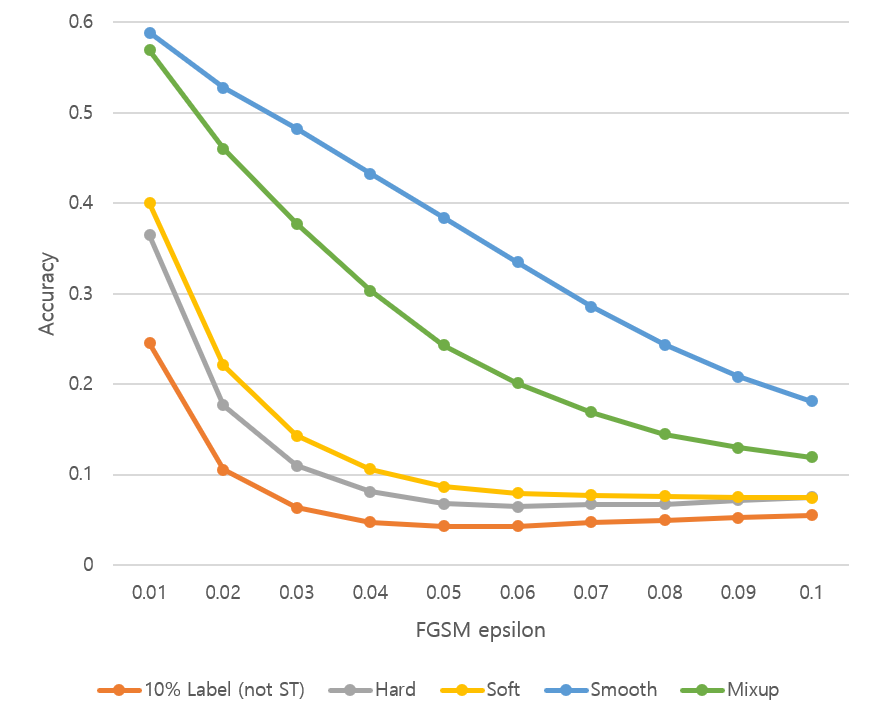
\includegraphics[width=.6\textwidth]{resource/FGSM}
  \caption{각 pseudo label 타입별 FGSM adversarial attack에 대한 강직도 테스트. 주황색 데이터는 self-training을 거치지 않은 ResNet-38 데이터이다.}
  \label{fgsm}
\end{figure}
위 방식으로 공격 이미지 $\vec x'$를 만들었다. 여기서 $\epsilon$은 공격의 강도로
취급할 수 있으며, 나는 이 공격을 이미지의 각 픽셀 RGB 값을 $[0, 1]$ 범위 값으로
바꾼 상태에서 적용하였다.
그림 \ref{fgsm}에서 같이 초기 teacher model에 비해서 더 높은 강직도를 획득했음을
알 수 있었다. Hard보다는 soft가, 그리고 그것보다 mixup과 label smoothing이 훨씬
좋았다. \cite{goibert2019adversarial}와 \cite{zhang2018mixup}에서 언급했던 두
방법의 강직성이 noisy student 방식에서도 그대로 나타났다.

\subsection{Calibration Errors \& Robustness on Corruptions/Perturbations}
Calibration error와 다른 여러 지표들도 분석해보았다. Calibration error란 모델이
예측한 confidence 값과 실제 accuracy가 얼마나 차이가 있는지 확인하는 지표로,
모델의 overconfident 문제를 진단할 수 있다. \cite{guo2017calibration} 보통
ECE(expected calibration error)로 측정한다. Confidence 결과를 $0.1$ 단위로 총
10개의 묶음으로 쪼개어, 각 묶음 별로 실제 accuracy와 confidence의 평균이 얼마나
차이가 나며, 그 차이의 평균을 나타내는 지표이다. ECE 값이 차이가 적게 나야
중요한 의사 결정에서 모델이 말하는 confidence를 신뢰할 수 있을 것이므로 좋은
모델이라고 간주할 수 있다.

또한 CIFAR-10 이미지를 corruption 시킨 CIFAR-10-C 데이터셋과, perturbation 시킨
CIFAR-10-P 데이터셋을 구하여 돌려보기도 하였다. 둘은
\cite{hendrycks2019benchmarking}에서 제안된 데이터로, 실제 이미지 분류 문제에서
자주 직면하는 여러 오염적인 상황들이 적용된 이미지를 테스트하는데 사용한다. 본래
ImageNet-C, ImageNet-P가 더 보편적이지만, 본 프로젝트에서 학습한 데이터가
CIFAR-10이므로, 이를 오염시킨 데이터셋으로 실험하였다. 

ImageNet-C에서는 각 오염 요소에 따른 5개의 강도마다 CE(corruption error)를
구하고, 이를 기준 네트워크인 AlexNet과 비교를 통해 relative mCE(mean CE)를
계산하여 오염에 대한 강직성을 수치화시킨다. \cite{hendrycks2019benchmarking}
\begin{align*}
  CE_{c}^f &= \frac{\left( \sum_{s=1}^5 E_{s,c}^f - E_{clean}^f \right)}
  {\left( \sum_{s=1}^5 E_{s,c}^{AlexNet} - E_{clean}^{AlexNet} \right)} \\
  mCE^f &= \frac{1}{|C|} \sum_{c \in C} CE_{c}^f
\end{align*}
또한, ImageNet-P에서는 각 오염 요소마다, 오염 요소의 강도별로 얼마나 많은 예측
결과들이 달라지는지 FP(flip probability)를 통해 강직성을 검사한다. 이 또한 각
perturbation에 대해 기준 네트워크인 AlexNet과 비율을 계산하여 평균을 내는
방식으로 mFP(mean FP)를 계산하여 수치화시킨다. \cite{hendrycks2019benchmarking}
\begin{align*}
  FP_{p}^f &= \frac{1}{m(n-1)} \sum_{i=1}^m \sum_{j=2}^n \vec{1}
  \left( f(x_j^{(i)}) \neq f(x_j^{(1)}) \right) \\
  mFP^f &= \frac{1}{|P|} \sum_{p \in P} \frac{FP_p^f}{FP_p^{AlexNet}}
\end{align*}
문제는 ImageNet에서 AlexNet과 달리 CIFAR-10 문제의 준 지도학습 결과에 대한 기준
네트워크 정보가 없다는 것이다. 그래서 나는 이 프로젝트에서 대조군으로 사용하기
위해 self-training 없이 5,000개의 training data로 학습한 ResNet-38을 기준
네트워크로 설정하여 위 수치들을 계산해보았다.
\begin{table}[!h]
  \center
  \begin{tabular}{ |c|c|c|c|c|c| }
    \hline
      Label Type & Network & Top-1 Acc. & ECE & Rel. mCE & mFR \\ \hline
      Teacher & ResNet-20 & 82.27 & 0.1142 & 117.29 & 105.90 \\ \hline
      Hard & ResNet-26 & 86.36 & 0.0762 & 103.10 & 86.18 \\ 
       & ResNet-32 & 87.58 & 0.0954 & 87.36 & 82.64 \\ 
       & ResNet-38 & 88.28 & 0.0814 & 75.61 & 75.11 \\ \hline
      Soft & ResNet-26 & 86.03 & 0.0494 & 77.16 & 85.51 \\
       & ResNet-32 & 87.68 & 0.0355 & 56.54 & 77.60 \\ 
       & ResNet-38 & 88.21 & 0.0495 & 72.95 & 70.16 \\ \hline
      Smooth & ResNet-26 & 86.19 & 0.0328 & 66.30 & 81.52 \\
       & ResNet-32 & 87.73 & 0.0504 & 74.72 & 78.07 \\ 
       & ResNet-38 & 88.48 & 0.0789 & 76.94 & 73.39 \\ \hline
      Mixup & ResNet-26 & 86.34 & 0.1056 & 60.31 & 83.91 \\
       & ResNet-32 & 86.70 & 0.0263 & 68.51 & 80.07 \\ 
       & ResNet-38 & 87.78 & 0.0780 & 50.11 & 75.58 \\ \hline
      Without ST & ResNet-38 & 83.91 & 0.1169 & 100.00 & 100.00 \\ \hline
  \end{tabular}    
  \caption{각 pseudo label 타입별 calibration error 및 corruption/perturbation robustness 지표. Top-1 accuracy 외 모두 낮은 수치가 좋다.}
  \label{robustness}
\end{table}

표 \ref{robustness}와 같이 결과가 나타났다. 우선 calibration error의 경우 모두
마지막 네트워크에서 ECE $0.1$ 이내의 준수한 값이 나타났으며, soft label에서 가장
적었다. 반면 overconfident 문제를 초래할 것으로 예측되었던 hard label에서 가장
높게 나타났지만, 여전히 원래 방식보다 적은 수치였다. Relative mCE의 경우 hard,
soft, smooth label에서는 비슷한 값이 나타났지만, mixup 방식에서 압도적으로 높은
성능이 보였다. 하지만 mFR의 경우 soft가 미세한 차이로 좋았지만, 여러 모델 간의
큰 차이는 도드라지지 않았다. 이를 통해 soft label, mixup 방식이 비교적 적은 수의
pseudo label 정보를 받았다는 점에서 top-1 accuracy를 내는 것에는 불리했지만, 더
overconfident 문제에서 자유로우며, 강직성이 높은 모델을 학습했음을 추론할 수
있었다.

\section{Ablation Studies}
\subsection{Effect of Noise Injections}
ImageNet과 같이 커다란 규모의 데이터셋과 네트워크가 필요한 학습에는 noise의
기여가 굉장히 크다는 사실에 공감할 수 있었다. \cite{xie2020selftraining} 하지만
나는 CIFAR-10과 같이 해상도가 낮고, ResNet-38과 같이 규모가 작은 네트워크에도
이것들이 유용한지 확인해보고 싶었다. 왜냐하면 해상도가 낮은 이미지는 같은
input noise에 대해 유실하는 중요한 정보의 비율이 높을 가능성이 있으며, model
noise가 모델의 representability를 축소시켜 학습 효과를 저해할 수도 있다는 생각이
들었기 때문이다. 그래서 나는 각 noise의 정도를 수정하거나 아예 없애는 방식이
학습 과정에 어떤 영향을 주는지 몇 가지 테스트를 해보았다.

표 \ref{ablation_noise}를 보자. 우선 input noise에 해당하는 RandAugment는 강도
27에서 가장 높은 top-1 정확도를 얻을 수 있었으며, 이것이 줄어들수록 더
낮아졌음을 알 수 있었다. 또한 ECE, relative mCE, mFR과 같은 거의 모든 지표에서
강도가 강해짐에 따라 더 좋은 수치가 나타나는 것으로 나타났다. 이로써 input
noise가 더 좋은 학습 과정을 유도하는데 크게 기여했음을 알 수 있었다.

하지만 model noise에 대해서는 다소 실망스러운 결과가 나타났다. 오히려 dropout을
없애는 편이 모든 수치에서 더 나은 결과를 가져왔다. Stochastic depth를 지웠을
때 relative mCE에서 robustness가 약간 깨졌지만, 대부분의 수치가 default보다 더
좋았다. 심지어 model noise를 아예 없애는 편이 거의 모든 수치에서 가장 뛰어났다.
이로써 내가 우려하던 model의 크기가 너무 작다는 가설이 어느 정도 맞았음을 알 수
있었다. 원 논문 \cite{xie2020selftraining}의 저자가 말했듯 student에게 ensemble
역할을 기대하는 것은, 이 정도 규모의 네트워크에서 무리였던 것 같다.

한 가지 신기했던 결과는, 모든 noise를 없앤 방법이 가장 나쁜 모델을 학습했다는
것이었다. 분명 RandAugment가 있는 상황에서 model noise를 제거하는 것은 긍정적인
결과를 가져왔지만, input noise가 없을 때 제거하는 것은 더 안 좋았다. Student
model에 noise가 하나도 없다면 이는 teacher model이 생성한 pseudo label 정보를
곧이 곧대로 수용한 격이 된다. 그래서 네트워크 규모의 팽창에도 불구하고 여러
지표의 향상이 전혀 나타나지 않고, 정답률도 84\%대에 머물렀던 것으로 판단된다.

결국 student model에 noise injection은 필수적이지만, 이를 효과적으로 적용하기
위해서는 underfitting 문제를 겪지 않도록 충분히 representability가 큰 네트워크로
학습해야한다는 사실을 추론할 수 있었다.

\begin{table}[!h]
  \center 
  \begin{tabular}{|c|c|c|c|c|c|}
    \hline
      Noise Injections & Network & Top-1 Acc. & ECE & Rel. mCE & mFR \\ \hline
      Default & ResNet-26 & 86.36 & 0.0762 & 103.10 & 86.18 \\
       & ResNet-32 & 87.58 & 0.0954 & 87.36 & 82.64 \\
       & ResNet-38 & 88.28 & 0.0814 & 75.61 & 75.11 \\ \hline
      RandAugment 3 & ResNet-26 & 85.87 & 0.0435 & 105.32 & 95.72 \\
       & ResNet-32 & 86.84 & 0.1221 & 72.51 & 88.78 \\
       & ResNet-38 & 87.22 & 0.0989 & 124.61 & 87.45 \\ \hline
      RandAugment 9 & ResNet-26 & 85.84 & 0.0796 & 86.25 & 96.17 \\
       & ResNet-32 & 87.02 & 0.1050 & 108.20 & 89.26 \\
       & ResNet-38 & 87.77 & 0.1012 & 97.12 & 88.00 \\ \hline
      No RandAugment & ResNet-26 & 85.33 & 0.0842 & 133.48 & 105.97 \\
       & ResNet-32 & 86.10 & 0.1335 & 152.33 & 109.73 \\
       & ResNet-38 & 86.37 & 0.1141 & 119.29 & 110.19 \\ \hline
      Dropout 0.2 & ResNet-26 & 86.60 & 0.0473 & 115.74 & 84.83 \\
       & ResNet-32 & 88.40 & 0.0810 & 78.71 & 73.46 \\
       & ResNet-38 & 88.69 & 0.1002 & 88.91 & 69.61 \\ \hline
      No Dropout & ResNet-26 & 86.62 & 0.0656 & 99.11 & 83.59 \\
       & ResNet-32 & 88.26 & 0.0791 & 78.05 & 75.92 \\
       & ResNet-38 & 88.55 & 0.0926 & 52.11 & 73.98 \\ \hline
      No Stoch. Depth & ResNet-26 & 86.52 & 0.0934 & 79.60 & 84.62 \\
       & ResNet-32 & 87.81 & 0.1014 & 82.93 & 76.26 \\
       & ResNet-38 & 88.89 & 0.0942 & 86.92 & 74.20 \\ \hline
      No Model Noise & ResNet-26 & 86.53 & 0.0775 & 91.57 & 82.58 \\
       & ResNet-32 & 88.52 & 0.0847 & 102.00 & 75.25 \\
       & ResNet-38 & 88.74 & 0.0930 & 64.30 & 76.72 \\ \hline
      No Noise & ResNet-26 & 84.11 & 0.1318 & 154.32 & 111.06 \\
       & ResNet-32 & 84.35 & 0.1227 & 168.07 & 114.16 \\
       & ResNet-38 & 84.59 & 0.1305 & 164.30 & 110.77 \\ \hline
  \end{tabular}
  \caption{Noise injection별 모델 학습 결과. Default는 학습 기본 설정(stochastic depth, dropout=0.5, RandAugment 27)을 의미한다. Top-1 정확도 외 모두 낮을수록 좋다.}
  \label{ablation_noise}
\end{table}

\subsection{Effect of Confidence Threshold on Pseudo Label Generations}
Soft, label smoothing, mixup과 같은 방법을 사용하면 비교적 overconfident
문제에서 자유로워지는 대신, confidence threshold를 넘기는 데이터 수가 적어져
pseudo labeled data가 충분히 확보되지 않는 문제가 발생했다. 이에 대한 해결책으로
confidence threshold를 내리는 방법이 있다. 하지만 teacher가 생성한 pseudo
label에 대한 신뢰성은 더 떨어지므로 학습이 제대로 이루어지지 않을 가능성이 있다.
나는 그 중간선이 무엇인지 확인해보고 싶어서 confidence threshold를 0.7,
0.8(default), 0.9로 설정하고 결과를 관찰했다.
\begin{table}[!h]
  \center 
  \begin{tabular}{|c|c|c|c|c|c|c|}
    \hline
    Label Type & Conf. Thres. & Network & Top-1 Acc. & ECE & Rel. mCE & mFR \\ \hline
    Hard & 0.7 & ResNet-26 & 86.05 & 0.0675 & 80.27 & 80.98 \\
     &  & ResNet-32 & 87.49 & 0.0874 & 78.05 & 79.77 \\
     &  & ResNet-38 & 88.36 & 0.0959 & 88.69 & 73.03 \\ \hhline{|~|-|-|-|-|-|-|}
     & 0.8 & ResNet-26 & 86.05 & 0.0675 & 80.27 & 80.98 \\
     &  & ResNet-32 & 87.49 & 0.0874 & 78.05 & 79.77 \\
     &  & ResNet-38 & 88.36 & 0.0959 & 88.69 & 73.03 \\ \hhline{|~|-|-|-|-|-|-|}
     & 0.9 & ResNet-26 & 86.83 & 0.0686 & 97.56 & 85.72 \\
     &  & ResNet-32 & 88.01 & 0.0728 & 88.25 & 75.69 \\
     &  & ResNet-38 & 88.78 & 0.1028 & 42.13 & 71.87 \\ \hline
    Soft & 0.7 & ResNet-26 & 86.25 & 0.0354 & 117.07 & 89.46 \\
     &  & ResNet-32 & 87.19 & 0.0628 & 94.24 & 77.76 \\
     &  & ResNet-38 & 88.36 & 0.0574 & 79.38 & 75.43 \\ \hhline{|~|-|-|-|-|-|-|}
     & 0.8 & ResNet-26 & 86.03 & 0.0494 & 77.16 & 85.51 \\
     &  & ResNet-32 & 87.68 & 0.0355 & 56.54 & 77.60 \\
     &  & ResNet-38 & 88.21 & 0.0495 & 72.95 & 70.16 \\ \hhline{|~|-|-|-|-|-|-|}
     & 0.9 & ResNet-26 & 86.46 & 0.0569 & 106.21 & 83.72 \\
     &  & ResNet-32 & 87.99 & 0.0894 & 77.83 & 76.24 \\
     &  & ResNet-38 & 88.52 & 0.0800 & 64.08 & 72.54 \\ \hline
    Smooth & 0.7 & ResNet-26 & 86.56 & 0.0310 & 104.66 & 84.34 \\
     &  & ResNet-32 & 87.47 & 0.0526 & 89.36 & 77.44 \\
     &  & ResNet-38 & 88.25 & 0.0628 & 52.77 & 74.17 \\ \hhline{|~|-|-|-|-|-|-|}
     & 0.8 & ResNet-26 & 86.19 & 0.0328 & 66.30 & 81.52 \\
     &  & ResNet-32 & 87.73 & 0.0504 & 74.72 & 78.07 \\
     &  & ResNet-38 & 88.48 & 0.0789 & 76.94 & 73.39 \\ \hhline{|~|-|-|-|-|-|-|}
     & 0.9 & ResNet-26 & 86.99 & 0.0357 & 88.25 & 80.61 \\
     &  & ResNet-32 & 86.93 & 0.0494 & 91.57 & 83.67 \\
     &  & ResNet-38 & 88.12 & 0.0663 & 92.24 & 72.78 \\ \hline
    Mixup & 0.7 & ResNet-26 & 86.18 & 0.0777 & 67.85 & 84.63 \\
     &  & ResNet-32 & 86.90 & 0.0379 & 68.29 & 77.12 \\
     &  & ResNet-38 & 87.74 & 0.0369 & 70.51 & 75.86 \\ \hhline{|~|-|-|-|-|-|-|}
     & 0.8 & ResNet-26 & 86.34 & 0.1056 & 60.31 & 83.91 \\
     &  & ResNet-32 & 86.70 & 0.0263 & 68.51 & 80.07 \\
     &  & ResNet-38 & 87.78 & 0.0780 & 50.11 & 75.58 \\ \hhline{|~|-|-|-|-|-|-|}
     & 0.9 & ResNet-26 & 86.18 & 0.0539 & 56.98 & 86.06 \\
     &  & ResNet-32 & 86.68 & 0.1223 & 66.30 & 83.74 \\
     &  & ResNet-38 & 86.75 & 0.0682 & 55.65 & 85.44 \\ \hline
  \end{tabular}
  \caption{각 pseudo label 타입과 confidence threshold별 학습 모델 분석 결과. Top-1 accuracy를 제외하고는 모두 낮은 수치가 좋다.}
  \label{ablation_confidence}
\end{table}

표 \ref{ablation_confidence}를 살펴보자. Hard label의 경우 0.9인 상황에서 가장
우수한 top-1 정확도와 앞도적으로 낮은 relative mCE 값을 얻어낼 수 있었다.
Overconfident 문제를 보이는 만큼 대부분의 라벨이 높은 confidence로 분류되어
pseudo label이 부족하게 제작되지 않았으며, 따라서 더 신뢰도 있는 데이터를
학습함으로써 나타나는 긍정적인 효과들이 더 두드러졌다.

반면 soft label의 경우 낮은 threshold가 0.9보다 약간 더 나은 결과를 가져왔다.
비록 Top-1 정확도는 0.9가 가장 높긴 했지만(88.52\%) 큰 차이는 아니었고, ECE 값이
threshold가 낮을수록 더 안정되었다. 애초에 soft label은 model 계산의 최대값을
보는게 아니라 confidence 자체를 학습하므로 threshold 문제에서 자유로우며, 때문에
threshold를 낮췄을 때 더 많은 이미지를 학습하여 이득을 보았던 것으로 판단된다.

\begin{table}[!h]
  \center
  \begin{tabular}{|c|c|cccccccccc|}
\hline
Conf. Thres. & Network & airp. & autom. & bird & cat & deer & dog & frog & horse & ship & truck \\ \hline
0.7 & ResNet-20 & 4411 & 4742 & 4578 & 4638 & 4668 & 3922 & 4465 & 4390 & 4851 & 4628 \\
    & ResNet-26 & 4177 & 4716 & 4171 & 4060 & 4631 & 3424 & 4242 & 4165 & 4853 & 4593 \\
    & ResNet-32 & 4450 & 4846 & 4399 & 4672 & 4972 & 3980 & 4507 & 4399 & 5013 & 4700 \\ \hline

0.8 & ResNet-20 & 4236 & 4673 & 4301 & 4248 & 4430 & 3621 & 4313 & 4226 & 4691 & 4508 \\ 
    & ResNet-26 & 4046 & 4635 & 3864 & 3344 & 4235 & 3114 & 3997 & 4027 & 4610 & 4494 \\
    & ResNet-32 & 4330 & 4781 & 4319 & 4045 & 4455 & 3824 & 4278 & 4212 & 4734 & 4620 \\ \hline

0.9 & ResNet-20 & 3951 & 4551 & 3922 & 3684 & 4098 & 3240 & 4081 & 4038 & 4491 & 4335 \\ 
    & ResNet-26 & 3610 & 4510 & 3603 & 2546 & 3883 & 2580 & 3639 & 3628 & 4287 & 4172 \\
    & ResNet-32 & 3648 & 4406 & 3661 & 2512 & 3239 & 2233 & 3712 & 3102 & 3999 & 3916 \\ \hline
  \end{tabular}
  \caption{Label smoothing 방식. 각 confidence threshold에 따라 teacher model이 생성한 클래스별 학습 데이터의 개수}
  \label{datagen_smooth_confidence}
\end{table}
\begin{table}[!h]
  \center
  \begin{tabular}{|c|c|cccccccccc|}
\hline
Conf. Thres. & Network & airp. & autom. & bird & cat & deer & dog & frog & horse & ship & truck \\ \hline
0.7 & ResNet-20 & 4411 & 4742 & 4578 & 4638 & 4668 & 3922 & 4465 & 4390 & 4851 & 4628 \\
    & ResNet-26 & 4028 & 4506 & 3357 & 2994 & 3531 & 2797 & 3695 & 3762 & 4333 & 4212 \\
    & ResNet-32 & 4432 & 4726 & 4043 & 3911 & 3997 & 3594 & 4157 & 4135 & 4599 & 4489 \\ \hline

0.8 & ResNet-20 & 4236 & 4673 & 4301 & 4248 & 4430 & 3621 & 4313 & 4226 & 4691 & 4508 \\ 
    & ResNet-26 & 2926 & 2999 & 2110 & 1759 & 1863 & 1703 & 1476 & 2036 & 3342 & 2853 \\
    & ResNet-32 & 3999 & 4451 & 3521 & 3301 & 3466 & 3360 & 3747 & 3731 & 4281 & 4288 \\ \hline

0.9 & ResNet-20 & 3951 & 4551 & 3922 & 3684 & 4098 & 3240 & 4081 & 4038 & 4491 & 4335 \\ 
    & ResNet-26 & 2662 & 1685 & 1870 & 1464 & 1427 & 1346 & 1190 & 1398 & 2979 & 2055 \\
    & ResNet-32 & 801 & 575 & 594 & 580 & 530 & 538 & 538 & 531 & 838 & 568 \\ \hline 
  \end{tabular}
  \caption{Mixup 방식. 각 confidence threshold에 따라 teacher model이 생성한 클래스별 학습 데이터의 개수}
  \label{datagen_mixup_confidence}
\end{table}
또한 label smoothing과 mixup 방식에서는 도무지 규칙을 이해할 수 없는 결과가
나타났다. 이를 제대로 고찰하기 위해 각 단계에서 몇 개의 pseudo labeled data를
생성하는지 진단해보았다. 표 \ref{datagen_smooth_confidence}에서와 같이 label
smoothing 방식에는 threshold가 0.7, 0.8인 상황에 대해 pseudo label이 매 단계마다
제대로 생성되었음을 확인할 수 있었다. 하지만 0.9인 상황에서는 부실하게
형성되었으며, 따라서 top-1 정확도가 가장 낮았다. 이는 우리가 label smoothing에
사용한 $\epsilon$ 값이 $0.9$였으며, 때문에 가장 강력한 output signal이 이 정도
값에 수렴하여 너무 많은 데이터가 무의미하게 걸러졌기 때문인 것으로 판단된다. 표
\ref{datagen_mixup_confidence}에서 mixup 방식이 pseudo label 데이터를 얼마나
생성하는지 확인했다. Threshold 0.7인 상황에서는 충분히 많은 데이터가
생성되었으나, 낮은 신뢰도 문제로 인해 0.8보다 더 학습도가 떨어졌으며 relative
mCE와 같은 수치가 더 높게 나타났다. Threshold 0.9인 상황에서는 마치 mixup+soft
label과 같은 상황처럼 부실한 데이터가 형성되어 학습도가 떨어졌으나, 있는
데이터에 대한 신뢰도는 높아 relative mCE와 같은 수치가 좋았음을 알 수 있었다.
이와 같이 confidence threshold를 올리거나 내리는 상황에서 발생하는 여러
tradeoff들을 관찰할 수 있었다.

\subsection{Effect of Labeled Data Ratio}
나는 초기 학습 데이터의 10\%만 label을 유지하는 방식으로 준 지도학습 상황을
구성했다. 이 비율을 수정했을 때 학습 결과는 어떻게 달라지는지 궁금증이 생겼다.
결국 labeling을 하는 작업은 시간과 돈을 소모하는 작업인데, 이에 대한 효용을
측정할 수 있기 때문이다.
\begin{table}[!h]
  \center 
  \begin{tabular}{|c|c|c|c|c|c|c|}
    \hline
    Label Type & Init. Label & Network & Top-1 Acc. & ECE & Rel. mCE & mFR \\ \hline
    Hard & 5\% & ResNet-38 & 85.83 & 0.1117 & 27.27 & 78.76 \\
     & 10\% & ResNet-38 & 88.28 & 0.0814 & 75.61 & 75.11 \\
     & 20\% & ResNet-38 & 89.63 & 0.0873 & 58.09 & 67.88 \\ \hline
    Soft & 5\% & ResNet-38 & 86.00 & 0.0828 & 54.32 & 82.94 \\
     & 10\% & ResNet-38 & 88.21 & 0.0495 & 72.95 & 70.16 \\
     & 20\% & ResNet-38 & 89.78 & 0.0628 & 75.39 & 67.52 \\ \hline
    Smooth & 5\% & ResNet-38 & 86.22 & 0.0857 & 59.42 & 78.17 \\
     & 10\% & ResNet-38 & 88.48 & 0.0789 & 76.94 & 73.39 \\
     & 20\% & ResNet-38 & 89.56 & 0.0523 & 64.97 & 68.76 \\ \hline
    Mixup & 5\% & ResNet-38 & 85.42 & 0.0723 & 38.80 & 89.66 \\
     & 10\% & ResNet-38 & 87.78 & 0.0780 & 50.11 & 75.58 \\
     & 20\% & ResNet-38 & 88.70 & 0.0826 & 74.06 & 72.23 \\ \hline
  \end{tabular}    
  \caption{각 pseudo label 타입별 robustness 및 calibration error 지표. Top-1 accuracy를 제외하고는 모두 낮은 수치가 좋다.}
  \label{ratio}
\end{table}
표 \ref{ratio}에서 나타나는 것과 같이 모든 pseudo label 방식에서 초기 labeled
비율이 높을수록 더 큰 top-1 정확도가 나옴을 관찰할 수 있었다. 특히 soft label의
경우 20\% 비율 시작점에서 거의 90\%에 근접하는 수치가 나타났다. 그러므로
CIFAR-10과 같이 전체 데이터의 수가 적은 상황에서는 최대한 많은 labeled data를
확보하는 과정이 유의미한 효용을 준다는 것을 깨달았다.

비교적 낮은 5\% labeled training set 상황에서 label smoothing 방식이 가장
뛰어났는데, teacher model이 생성한 pseudo label을 신뢰하지 못하는 상황이기
때문인 것으로 파악된다. 또한 5\% 상황에서 비정상적으로 낮은 수준의 relative
mCE가 관찰되었다. 각 corruption 별 정답율을 살펴보았다. 이들은 애초에 clean
image에 대한 accuracy부터 너무 낮으며, 애초에 어려운 데이터를 이미 clean
image에서 다 틀렸기 때문에 $E_{s,c}^f - E_{clean}^f$ 항이 비교적 작게 나와서
그런 것으로 파악되었다.


\section{Conclusion}
이번 프로젝트를 통하여 \cite{xie2020selftraining} 논문에 있는 teacher-noisy
student models self-training을 CIFAR-10 데이터셋에 대해 구현해보았다. 논문에
나오는 내용과 더불어 label smoothing, mixup과 같은 응용적인 pseudo label 생성
방법을 적용해보았으며, 학습된 모델 결과를 여러 지표에 따라 분석해볼 수 있었다.
그 과정에서 label smoothing, mixup이 FGSM과 같은 adversarial attack에 강직하며,
mixup은 relative mCE 수치가 가장 뛰어나 오염에 강직하다는 사실을 알게 되었다.
또한 초기 labeled data의 비율이 높을수록 더 뛰어난 모델을 학습할 수 있음을
깨달았으며, CIFAR-10과 같이 전체 이미지 수가 적은 경우에 대해서는 데이터
labeling 중노동이 의미있는 효과를 불러준다는 사실을 알 수 있었다.

하지만 CIFAR-10 데이터셋의 부족한 이미지 수와 비교적 작은 규모의 학습
네트워크로부터 여러 한계점을 관찰하기도 했다. Label smoothing이나 mixup을
사용하는 경우 overconfident 문제를 해결할 수 있지만, confidence threshold를
넘어가는 이미지 수가 적어져 많은 수의 pseudo label을 확보하기 어려웠다. 때문에
mixup은 hard label 이외 다른 방식과 결합하여 사용하는데 지장이 있었다. 그렇다고
confidence threshold를 조정하니 신뢰도가 낮은 저품질 데이터를 인수받거나 학습
데이터가 적어지는 등의 tradeoff가 명확히 드러났다. 모델 네트워크의 규모가 작아
model noise가 오히려 악영향을 주는 사태가 관찰되었으나, 신기하게도 student에
모든 noise를 제거하니 오히려 가장 낮은 성능이 나타나 `noisy student'라는 단어의
정당성을 확인하기도 하였다. 만약 STL-10과 같이 준 지도학습 목적으로 만들어진 큰
규모의 데이터셋을, 더 큰 네트워크 모델로, 더 많은 teacher-noisy student 연결로써
학습했다면 원 논문에 가까운 이상적인 결과를 얻어낼 수 있었을 것 같지만, 시간과
자원의 한계로 인해 그러지 못했던 사실이 아쉬웠다. 또한 같은 CIFAR-10 준 지도학습
데이터셋으로부터 다른 방식으로 학습한 모델과 여러 지표를 비교한다면 더 객관적인
분석이 가능했을 것 같지만(Robustness 향상이 self training 덕분인지, noise
injection 덕분인지 구분하기 등), 같은 이유로 수행하지 못해서 아쉬웠다.

처음으로 toy model에서 벗어나 제대로 돌려본 딥러닝 프로젝트였다. PyTorch 코드를
이렇게까지 사용해본적은 여태껏 없었다. 정말 사소한 것 하나 하나로 학습의
완성도가 크게 갈렸다. Optimizer의 종류, learning rate, 그리고 가장 중요한
scheduler 문제 때문에 초반에 엄청 고역을 겪었다. 여러 시행착오 끝에 감을
잡고나서 내 개인 소유의 데스크탑(AMD Ryzen 3700X, RTX 2070 Super)으로 학습을
돌렸는데, teacher를 제외하고 ResNet-26, 32, 38에 해당하는 student 학습시키는데만
약 3시간 정도의 시간이 소요되었다. 또한 학습이 끝난 뒤 이를 분석하는데도 많은
시간이 들어갔다. 특히 CIFAR-10-P의 경우 데이터 크기만 18GB가 넘어갔기 때문이다.
한 모델을 분석하는데 약 10분 정도가 소요되었다. 온갖 가설을 세우고 검증하느라 약
40세트의 student model을 학습해서, \texttt{run\_train.sh}, \texttt{run\_test.sh}
스크립트가 5-6일 내내 침대 옆에서 돌아가 따로 난방을 켜지 않아도 방 안이 따뜻해
좋았다. 프로젝트 코드를 직접 구현하는 과정에서 adversarial attack, calibration
error, corruption robustness 등 내가 잘 몰랐던 개념들을 습득하게 되었으며,
딥러닝 코드에 대한 (특히 텐서 연산) 커다란 매력을 알게 되어 재미있었다. 정말
보람찬 프로젝트였다.




\bibliographystyle{unsrt}
\bibliography{references}

\end{document}
